
% This LaTeX was auto-generated from MATLAB code.
% To make changes, update the MATLAB code and republish this document.

\documentclass{article}
\usepackage{graphicx}
\usepackage{color}

\sloppy
\definecolor{lightgray}{gray}{0.5}
\setlength{\parindent}{0pt}

\begin{document}

    
    
\subsection*{Contents}

\begin{itemize}
\setlength{\itemsep}{-1ex}
   \item 00 Settings - Clear Environment and change directory
   \item Q. 01 - Fetch Data
   \item Q. 02 and 03 - Apply HP Filter
   \item Q. 04 - Repeat for lambdas 0
   \item Q. 04 - Repeat for lambdas inf
   \item Q. 05 - Apply Log
   \item Q. 05 - Repeat for lambdas inf
   \item Q. 06 - Std Deviation
   \item Q. 07 - Cyclical Series
   \item Q. 08 - a)
   \item Q. 08 - a)
   \item Q. 08 b) normalizing
   \item Q. 08 c) compute growth
   \item sanity checks
   \item TODO:
\end{itemize}


\subsection*{00 Settings - Clear Environment and change directory}

\begin{par}
Requires: * MATLAB 2018b * Datafeed Toolbox
\end{par} \vspace{1em}
\begin{verbatim}
clear; close all; clc;

% Changing working directory to current script dir
tmp = matlab.desktop.editor.getActive;
cd(fileparts(tmp.Filename));
% add functions path
addpath('./functions/');
\end{verbatim}
\begin{par}
Change the current folder to the folder of this m-file.
\end{par} \vspace{1em}


\subsection*{Q. 01 - Fetch Data}

\begin{verbatim}
startDate = "01/01/1996";
endDate = "01/01/2018";

series = ["FRAPFCEQDSNAQ" "DEUPFCEQDSNAQ" "ITAPFCEQDSNAQ" ...
"CLVMNACSCAB1GQFR", "CLVMNACSCAB1GQDE", "CLVMNACSCAB1GQIT"];
\end{verbatim}
\begin{par}
Using `fred` and `fetch` function to retrieve data from FRED this function requires the Datafeed Toolbox. If toolbox is not available try to load the data that should be stored in a subfolder called 'data' with the following command:
\end{par} \vspace{1em}
\begin{verbatim}load('data/dataStruct.mat')\end{verbatim}
\begin{verbatim}
% using fred.stloisfed connection
url = "https://fred.stlouisfed.org/";

% retrieve data struct of the 6 time series
dataStruct = fetch(fred(url), series, startDate, endDate);

% consumption data
con_fr = dataStruct(1).Data(:,2);
con_de = dataStruct(2).Data(:,2);
con_it = dataStruct(3).Data(:,2);

% gdp data
gdp_fr = dataStruct(4).Data(:,2);
gdp_de = dataStruct(5).Data(:,2);
gdp_it = dataStruct(6).Data(:,2);
\end{verbatim}
\begin{par}
where: *  (:,2) : extract second column vector from *  the row caled 'Data', from *  the (1:6) row of object defined as dataStruct and *  define as con\_* and gdp\_* respectively
\end{par} \vspace{1em}
\begin{verbatim}
%%%% Transform Data

con_fr = con_fr / 10^9;
con_de = con_de / 10^9;
con_it = con_it / 10^9;

gdp_fr = gdp_fr / 10^3;
gdp_de = gdp_de / 10^3;
gdp_it = gdp_it / 10^3;
\end{verbatim}


\subsection*{Q. 02 and 03 - Apply HP Filter}

\begin{verbatim}
lambda = 1600;
rinseAndRepeat('gdp', gdp_fr, gdp_de, gdp_it, con_fr, con_de, con_it, lambda)
rinseAndRepeat('con', gdp_fr, gdp_de, gdp_it, con_fr, con_de, con_it, lambda)
\end{verbatim}

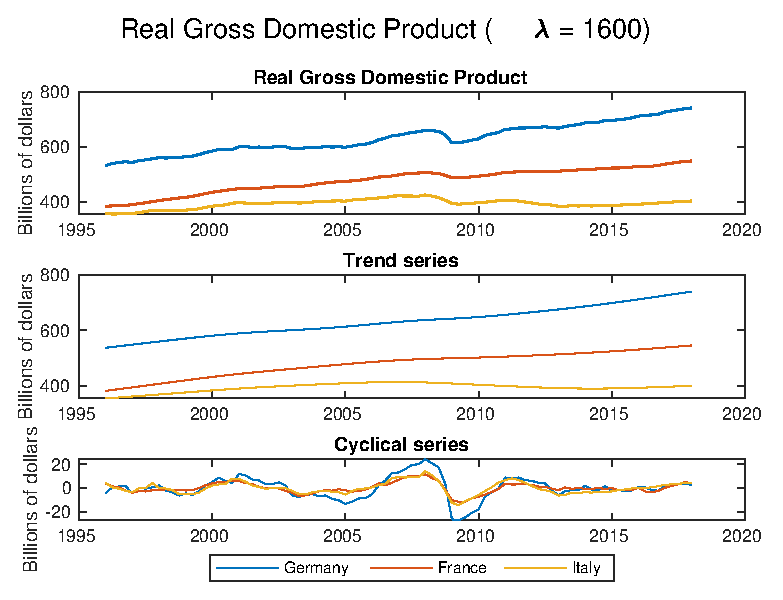
\includegraphics [width=4in]{assig01v01_01.eps}

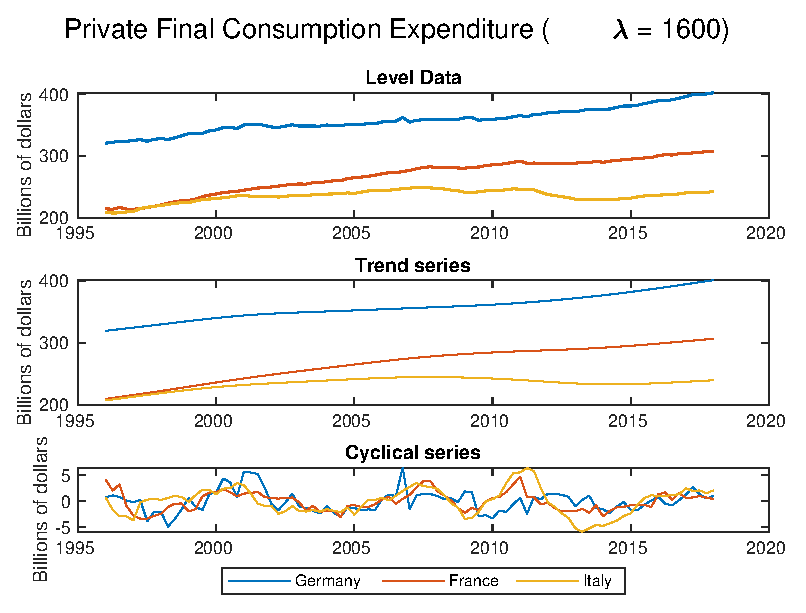
\includegraphics [width=4in]{assig01v01_02.eps}


\subsection*{Q. 04 - Repeat for lambdas 0}

\begin{verbatim}
%%%% lambda -> 0

lambda = 0;
rinseAndRepeat('gdp', gdp_fr, gdp_de, gdp_it, con_fr, con_de, con_it, lambda)
rinseAndRepeat('con', gdp_fr, gdp_de, gdp_it, con_fr, con_de, con_it, lambda)
\end{verbatim}

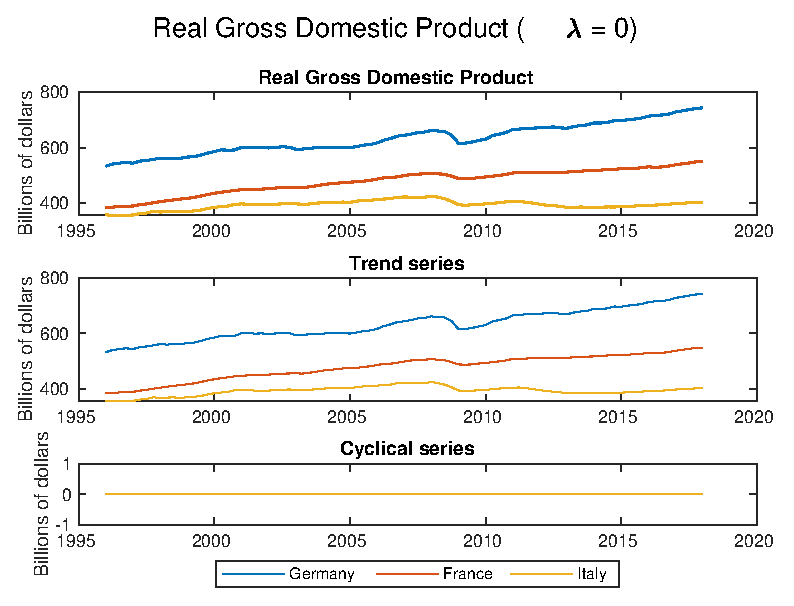
\includegraphics [width=4in]{assig01v01_03.eps}

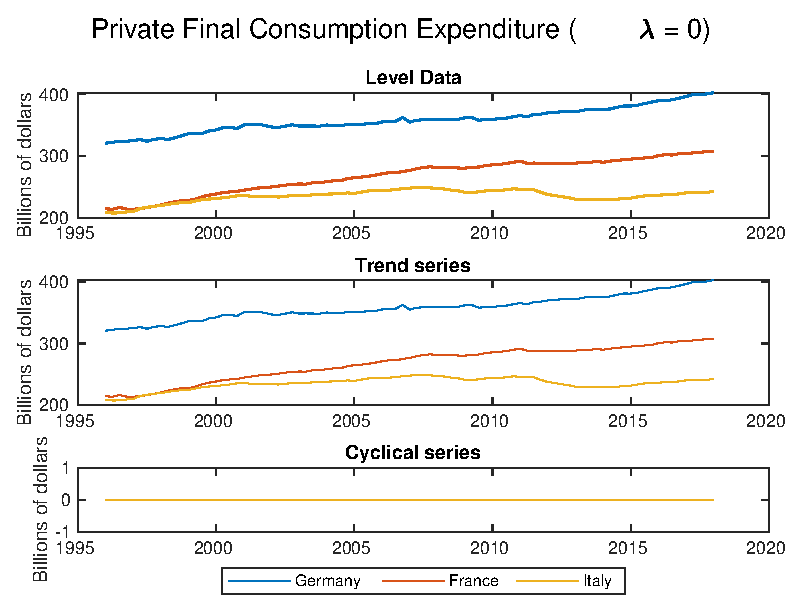
\includegraphics [width=4in]{assig01v01_04.eps}
\begin{par}
ANSWER: In this case we only minimize the first term of the HP-filter minimization problem. So the trend component is exactly the same as the observated data, and the cyclical component is, therefore, zero.
\end{par} \vspace{1em}


\subsection*{Q. 04 - Repeat for lambdas inf}

\begin{verbatim}
lambda = 10^10;
rinseAndRepeat('gdp', gdp_fr, gdp_de, gdp_it, con_fr, con_de, con_it, lambda)
rinseAndRepeat('con', gdp_fr, gdp_de, gdp_it, con_fr, con_de, con_it, lambda)
\end{verbatim}

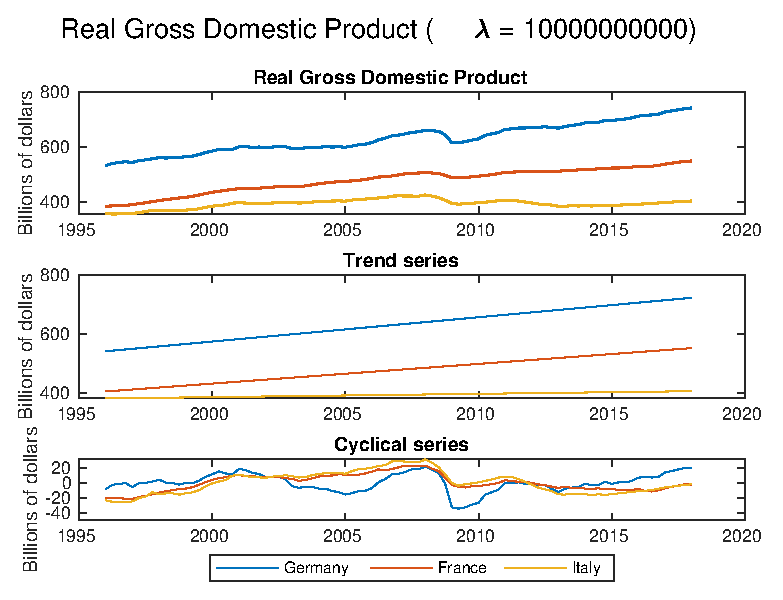
\includegraphics [width=4in]{assig01v01_05.eps}

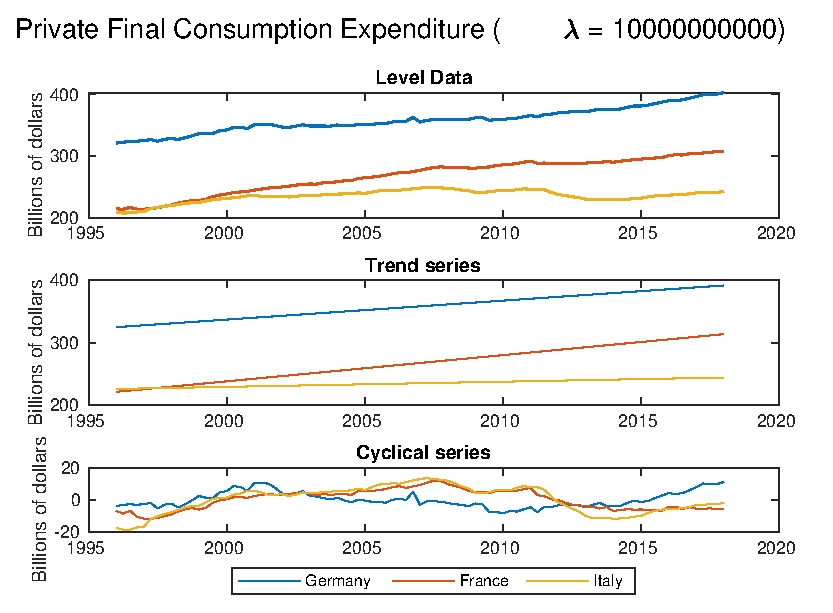
\includegraphics [width=4in]{assig01v01_06.eps}
\begin{par}
ANSWER: In the case of lambda -\ensuremath{>} inf, the second component in the HP-Filter gets the greatest weight and, therefore, we have a linear trend where the second term of the minization problem is zero, because the change in the trend is constant. The cyclical componente shows the difference between the observated data and the linear trend. Due to (near-) singularity problems, the matrix A from the HP-Filter function is not invertible for very big lambdas.  The results are, therefore, nonsensical and for Infitiy not computable.
\end{par} \vspace{1em}
\begin{verbatim}
lambda = 10^50;
rinseAndRepeat('gdp', gdp_fr, gdp_de, gdp_it, con_fr, con_de, con_it, lambda)
rinseAndRepeat('con', gdp_fr, gdp_de, gdp_it, con_fr, con_de, con_it, lambda)
\end{verbatim}

        \color{lightgray} \begin{verbatim}Warning: Matrix is close to singular or badly scaled. Results may be
inaccurate. RCOND =  1.505006e-18. 
Warning: Matrix is close to singular or badly scaled. Results may be
inaccurate. RCOND =  1.505006e-18. 
Warning: Matrix is close to singular or badly scaled. Results may be
inaccurate. RCOND =  1.505006e-18. 
Warning: Matrix is close to singular or badly scaled. Results may be
inaccurate. RCOND =  1.505006e-18. 
Warning: Matrix is close to singular or badly scaled. Results may be
inaccurate. RCOND =  1.505006e-18. 
Warning: Matrix is close to singular or badly scaled. Results may be
inaccurate. RCOND =  1.505006e-18. 
Warning: Matrix is close to singular or badly scaled. Results may be
inaccurate. RCOND =  1.505006e-18. 
Warning: Matrix is close to singular or badly scaled. Results may be
inaccurate. RCOND =  1.505006e-18. 
Warning: Matrix is close to singular or badly scaled. Results may be
inaccurate. RCOND =  1.505006e-18. 
Warning: Matrix is close to singular or badly scaled. Results may be
inaccurate. RCOND =  1.505006e-18. 
Warning: Matrix is close to singular or badly scaled. Results may be
inaccurate. RCOND =  1.505006e-18. 
Warning: Matrix is close to singular or badly scaled. Results may be
inaccurate. RCOND =  1.505006e-18. 
\end{verbatim} \color{black}
    
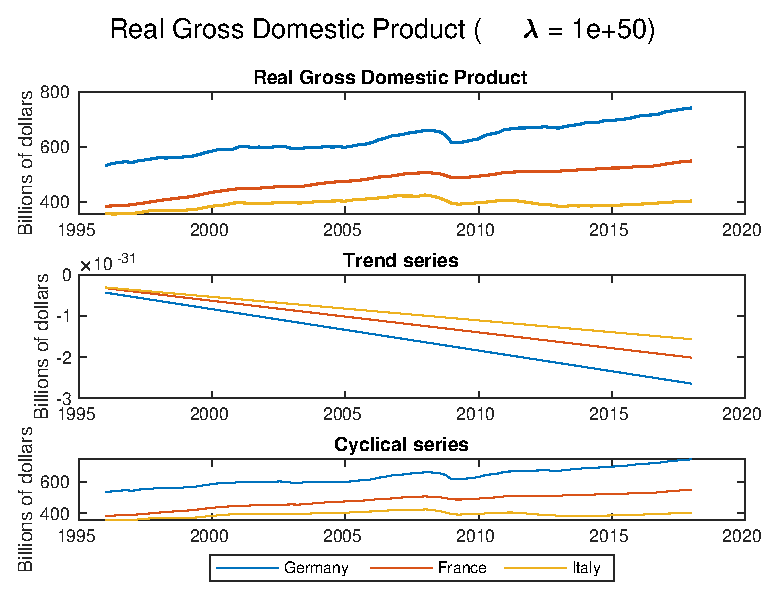
\includegraphics [width=4in]{assig01v01_07.eps}

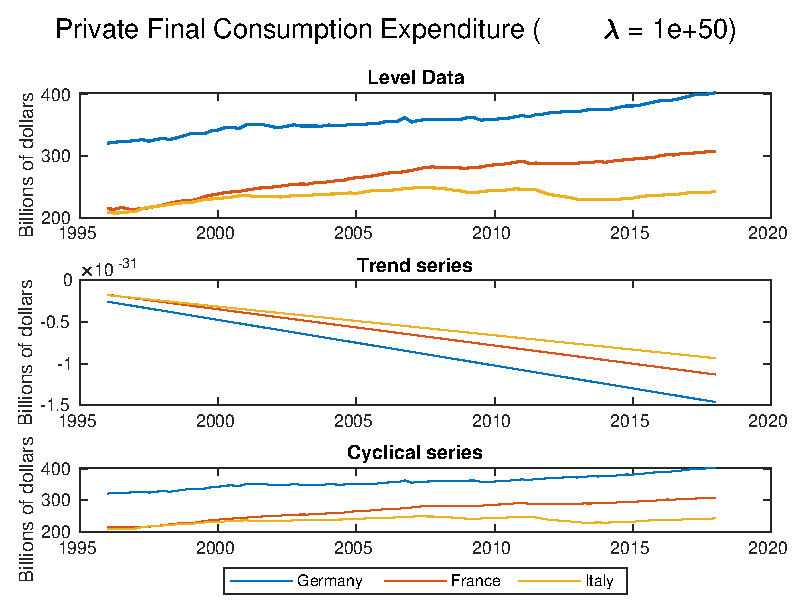
\includegraphics [width=4in]{assig01v01_08.eps}


\subsection*{Q. 05 - Apply Log}

\begin{verbatim}
lgdp_de = log(gdp_de);
lgdp_fr = log(gdp_fr);
lgdp_it = log(gdp_it);

lcon_de = log(con_de);
lcon_fr = log(con_fr);
lcon_it = log(con_it);

%%%% hp filter on log data
lambda = 1600;

[lgdp_T_fr, lgdp_C_fr] = hp_filter(lgdp_fr, lambda);
[lcon_T_fr, lcon_C_fr] = hp_filter(lcon_fr, lambda);

%%%% germany
[lgdp_T_de, lgdp_C_de] = hp_filter(lgdp_de, lambda);
[lcon_T_de, lcon_C_de] = hp_filter(lcon_de, lambda);

%%%% italy
[lgdp_T_it, lgdp_C_it] = hp_filter(lgdp_it, lambda);
[lcon_T_it, lcon_C_it] = hp_filter(lcon_it, lambda);
\end{verbatim}


\subsection*{Q. 05 - Repeat for lambdas inf}

\begin{verbatim}
close all
dates=1996.0:0.25:2018.0;

figure;
titleOfGraph = 'Cyclical Series (\lambda = ' + string(lambda) + ')';
sgtitle(titleOfGraph)
% working on 3 by 1 plots, plot 01
subplot(3,1,1);     % GERMANY
plot(dates, lgdp_C_de, 'LineWidth', 1); hold on;
plot(dates, lcon_C_de, 'LineWidth', 1); hold on;
xlabel('Years');
ylabel('Log Billions of dollars');
title('Germany');
legend('GDP', 'Consumptioin');

% working on 3 by 1 plots, plot 02
subplot(3,1,2);
plot(dates, lgdp_C_fr, 'LineWidth', 1); hold on;
plot(dates, lcon_C_fr, 'LineWidth',  1); hold on;
title('France');
ylabel('Log Billions of dollars');
xlabel('Years');

% working on 3 by 1 plots, plot 03
subplot(3,1,3)
plot(dates, lgdp_C_it, 'LineWidth', 1); hold on;
plot(dates, lcon_C_it, 'LineWidth', 1); hold on;
ylabel('Log Billions of dollars');
xlabel('Years');
title('Italy');
\end{verbatim}

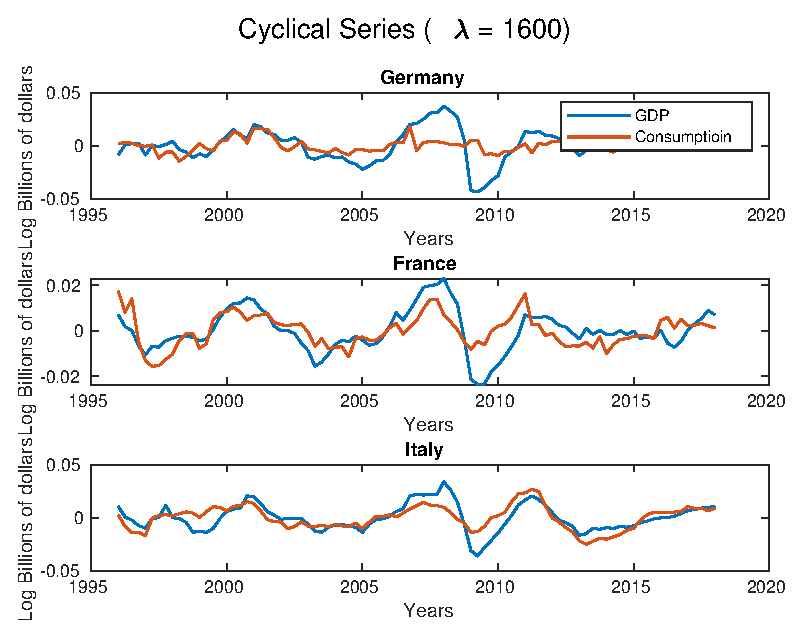
\includegraphics [width=4in]{assig01v01_09.eps}
\begin{par}
ANSWER: From the cyclical component above we can notice that GDP has a peak and declines sharply after the financial crises of 2007\ensuremath{\tilde{\;}}08. Especially for Italy one can notice the effects of the Euro sovereign debt crises around 2012. The cyclical series of consumption from Italy and France seem to closely follow the one of GDP. On the other hand, consumption in Germany is less affected by the strong changes in GDP. This could suggest that Households in Germany were less affected by both crises than in the other two countries.
\end{par} \vspace{1em}


\subsection*{Q. 06 - Std Deviation}

\begin{verbatim}
std(lgdp_C_de) %     0.0150
std(lgdp_C_fr) %     0.0092
std(lgdp_C_it) %     0.0128

std(lcon_C_de) %     0.0060
std(lcon_C_fr) %     0.0070
std(lcon_C_it) %     0.0110
\end{verbatim}

        \color{lightgray} \begin{verbatim}
ans =

    0.0150


ans =

    0.0092


ans =

    0.0128


ans =

    0.0060


ans =

    0.0070


ans =

    0.0110

\end{verbatim} \color{black}
    \begin{par}
ANSWER: The results show that consumption is less volatile than GDP in all three countries. This could be due to the fact that GDP absorbs also the volatility of its other components, that is, Gov't expenditure, Investments and Net Exports.
\end{par} \vspace{1em}
\begin{par}
The very low std deviation in consumption for Germany corroborates the hypothesis advanced in the previous answer.
\end{par} \vspace{1em}


\subsection*{Q. 07 - Cyclical Series}

\begin{verbatim}
%%%% Q.7 - a) slice timeseries

lambda = 1600;
startDate = 1996;
endDate = 2009;

lgdp_it_cut = timeseries(lgdp_it,dates);
lgdp_it_cut = getsampleusingtime(lgdp_it_cut, startDate, endDate);
lgdp_de_cut = timeseries(lgdp_de,dates);
lgdp_de_cut = getsampleusingtime(lgdp_de_cut, startDate, endDate);
lgdp_fr_cut = timeseries(lgdp_fr,dates);
lgdp_fr_cut = getsampleusingtime(lgdp_fr_cut, startDate, endDate);

[lgdp_it_cut_T, lgdp_it_cut_C] =  hp_filter(lgdp_it_cut.Data, lambda);
[lgdp_de_cut_T, lgdp_de_cut_C] =  hp_filter(lgdp_de_cut.Data, lambda);
[lgdp_fr_cut_T, lgdp_fr_cut_C] =  hp_filter(lgdp_fr_cut.Data, lambda);

%%%% Q.7 - a) plot cyclical series

datesCut = startDate:0.25:endDate;

figure;
% end-point

sgtitle('End-Points Bias')
% working on 3 by 1 plots, plot 01
subplot(3,1,1);
plot(dates, lgdp_C_de, 'LineWidth', 1)      ; hold on;
plot(datesCut, lgdp_de_cut_C, 'LineWidth', 1)  ; hold on;

xlabel('Years');
ylabel('Log Billions of dollars');
title('Germany');
legend('long', 'short');

% working on 3 by 1 plots, plot 01
subplot(3,1,2);
plot(dates, lgdp_C_fr, 'LineWidth', 1)      ; hold on;
plot(datesCut, lgdp_fr_cut_C, 'LineWidth', 1)  ; hold on;

xlabel('Years');
ylabel('Log Billions of dollars');
title('France');
legend('long', 'short');


subplot(3,1,3);
plot(dates, lgdp_C_it, 'LineWidth', 1)      ; hold on;
plot(datesCut, lgdp_it_cut_C, 'LineWidth', 1)  ; hold on;

xlabel('Years');
ylabel('Log Billions of dollars');
title('Italy');
legend('long', 'short');
\end{verbatim}

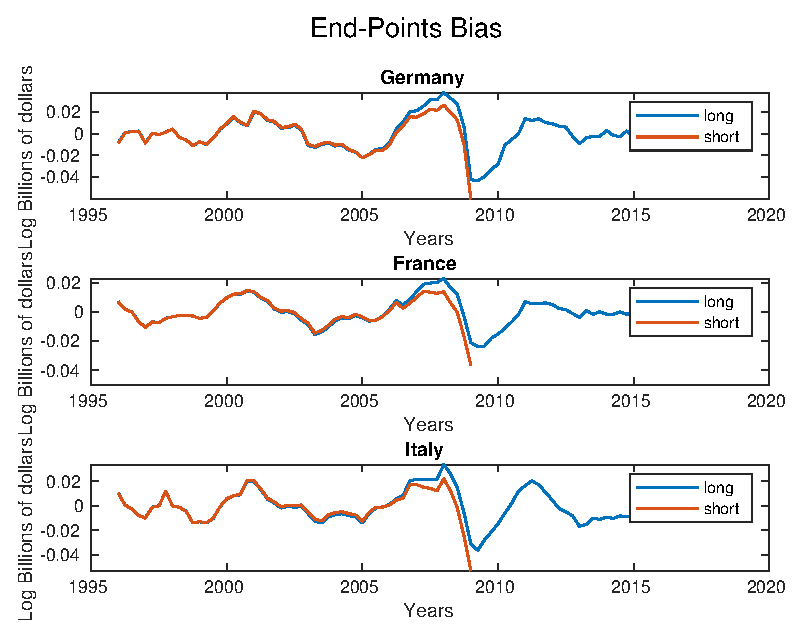
\includegraphics [width=4in]{assig01v01_10.eps}
\begin{par}
ANSWER: How one can take from the HP-Filter formula of the minimization problem, the first and the trend points, that is, the end-points, are not smoothed by the change in growth trend. That is, the second term is computed only from t=2 to T-1, whereas the first term is computed for the whole time series. This results in an exagerated estimation for the trend at the extremes. In our graph, one can see the bias only at the right end-point, because here we use the same starting date for the short and long series.
\end{par} \vspace{1em}
\begin{par}
Using the HP-Filter can be problematic when the (right) endpoint is the focus of the analysis and can lead to wrong inferences or predictions. Moreover, it is problematic because the endpoint bias reverberates not only on the very last points of the trend, but on a longer span, with dismishing impact towards the middle of the trend series.
\end{par} \vspace{1em}
\begin{verbatim}
figure;
plot(dates, lgdp_T_de, 'LineWidth', 1) ; hold on;
plot(datesCut, lgdp_de_cut_T, 'LineWidth', 1) ; hold on;
plot(dates, lgdp_de, 'LineWidth', 1); hold on;

xlabel('Years');
ylabel('Log Billions of dollars');
title('Germany');
legend('Location', 'northwest')
legend('long trend', 'end-point biased', 'log data');
\end{verbatim}

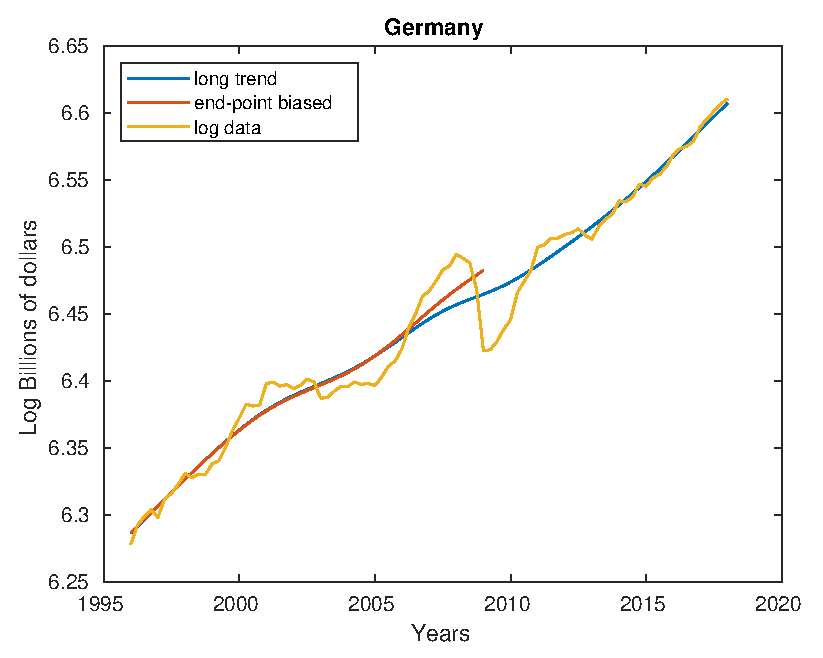
\includegraphics [width=4in]{assig01v01_11.eps}
\begin{par}
The direct effect of the endpoint bias can be more easily assessed when comparing the plot of the two trends, rather than the one of the resulting cyclical fluctuations. As one can see above, when dealing with the shorter time series, one overestimates the trend when compared to the longer time series.
\end{par} \vspace{1em}


\subsection*{Q. 08 - a)}

\begin{par}
Using `fred` and `fetch` function to retrieve data from FRED this function requires the Datafeed Toolbox. If toolbox is not available try to load the data that should be stored in a subfolder called 'data' with the following command:
\end{par} \vspace{1em}
\begin{verbatim}load('data/dataStruct.mat')\end{verbatim}
\begin{verbatim}
series = ["MKTGDPDEA646NWDB", "PCAGDPDEA646NWDB", ...
    "MKTGDPITA646NWDB", "PCAGDPITA646NWDB"];
startDate = "01/01/1970";
endDate = "01/01/2016";

% retrieve data struct of the 6 time series
url = "https://fred.stlouisfed.org/";
dataStruct2 = fetch(fred(url), series, startDate, endDate);

gdpDE = dataStruct2(1).Data(:,2);
gdpDEpc = dataStruct2(2).Data(:,2);
gdpIT = dataStruct2(3).Data(:,2);
gdpITpc = dataStruct2(4).Data(:,2);
\end{verbatim}


\subsection*{Q. 08 - a)}

\begin{verbatim}
lambda = 6.25;
[gdpDE_T, gdpDE_C] =  hp_filter(gdpDE, lambda);
[gdpDE_T_pc, gdpDEpc_C] =  hp_filter(gdpDEpc, lambda);

[gdpIT_T, gdpIT_C] =  hp_filter(gdpIT, lambda);
[gdpIT_T_pc, gdpITpc_C] =  hp_filter(gdpDEpc, lambda);
\end{verbatim}
\begin{par}
ANSWER: We picked \ensuremath{\backslash}lambda = 6.25, because it is the conventional value for annual data, whereas for quarterly it is 1600 and for monthly data. However, this is still a debated topic in the literature and some authors defend the usage of significantly different values, such as \ensuremath{\backslash}lambda = 100 for yearly data.
\end{par} \vspace{1em}


\subsection*{Q. 08 b) normalizing}

\begin{verbatim}
%germany
gdpDE_T_n = gdpDE_T / gdpDE_T(1);
gdpDE_T_n_pc = gdpDE_T_pc / gdpDE_T_pc(1);

% italy
gdpIT_T_n = gdpIT_T / gdpIT_T(1);
gdpIT_T_n_pc = gdpIT_T_pc / gdpIT_T_pc(1);


figure;
plot(dates, gdpIT_T, 'LineWidth', 1) ; hold on;
plot(dates, gdpIT, 'LineWidth', 1) ; hold on;
\end{verbatim}

        \color{lightgray} \begin{verbatim}Error using plot
Vectors must be the same length.

Error in assig01v01 (line 343)
plot(dates, gdpIT_T, 'LineWidth', 1) ; hold on;
\end{verbatim} \color{black}
    

\subsection*{Q. 08 c) compute growth}

\begin{verbatim}
%germany
DEgrowth =(gdpDE_T_n(2:end)./gdpDE_T_n(1:end-1)-1);
DEgrowth_pc =(gdpDE_T_n_pc(2:end)./gdpDE_T_n_pc(1:end-1)-1);

%italy
ITgrowth = (gdpIT_T_n(2:end)./gdpIT_T_n(1:end-1)-1);
ITgrowth_pc =(gdpIT_T_n_pc(2:end)./gdpIT_T_n_pc(1:end-1)-1);
\end{verbatim}
\begin{par}
Germay
\end{par} \vspace{1em}
\begin{verbatim}
%CAGR = (Ending value / Beginning value) ^ (1/n) - 1
CAGR_DE = (gdpDE_T_n(end) / gdpDE_T_n(1)) ^ (1 / length(gdpDE_T_n)) - 1
AAGR_DE = mean(DEgrowth)

CAGR_DE_pc = (gdpDE_T_pc(end) / gdpDE_T_pc(1)) ^ (1 / length(gdpDE_T_pc)) - 1
AAGR_DE_pc = mean(DEgrowth_pc)

% Italy
CAGR_IT = (gdpIT_T_n(end) / gdpIT_T_n(1)) ^ (1 / length(gdpIT_T_n)) - 1
AAGR_IT = mean(ITgrowth)

CAGR_IT_pc = (gdpIT_T_n_pc(end) / gdpIT_T_n_pc(1)) ^ (1 / length(gdpIT_T_n_pc)) - 1
AAGR_IT_pc = mean(ITgrowth_pc)
\end{verbatim}
\begin{par}
ANSWER: The compound average growth rate is: * 6.26\% for Germany's GDP * 6.16\% for Germany's GPD per capita, and * 6.26\% for Germany's GDP
\end{par} \vspace{1em}


\subsection*{sanity checks}

\begin{par}
Germany
\end{par} \vspace{1em}
\begin{verbatim}
gdpDE_T_n(1) * (1 + CAGR_DE) ^ length(gdpDE_T)
gdpDE_T_n(1) * (1 + AAGR_DE) ^ length(gdpDE_T)
gdpDE_T_n(end)

gdpDE_T_n_pc(1) * (1 + CAGR_DE_pc) ^ length(gdpDE_T_pc)
gdpDE_T_n_pc(1) * (1 + AAGR_DE_pc) ^ length(gdpDE_T_pc)
gdpDE_T_n_pc(end)


% Italy
gdpIT_T_n(1) * (1 + CAGR_IT) ^ length(gdpIT_T)
gdpIT_T_n(1) * (1 + AAGR_IT) ^ length(gdpIT_T)
gdpIT_T_n(end)

gdpIT_T_n_pc(1) * (1 + CAGR_IT_pc) ^ length(gdpIT_T_pc)
gdpIT_T_n_pc(1) * (1 + AAGR_IT_pc) ^ length(gdpIT_T_pc)
gdpIT_T_n_pc(end)
\end{verbatim}
\begin{verbatim}
figure;
dates = 1970:1:2016;
plot(dates, gdpIT_T_n); hold on;
plot(dates, gdpIT_T_n_pc); hold on;
\end{verbatim}
\begin{verbatim}
figure;
datesShort = 1971:1:2016;
plot(datesShort, ITgrowth); hold on;
plot(datesShort, ITgrowth_pc); hold on;
\end{verbatim}
\begin{verbatim}
plot(gdpDE)
title('ge')
\end{verbatim}
\begin{verbatim}
figure
plot(gdpDEpc)
title('ge pc')
\end{verbatim}
\begin{verbatim}
figure
plot(gdpIT)
title('it')
\end{verbatim}
\begin{verbatim}
figure
plot(gdpITpc)
title('it pc')
\end{verbatim}
\begin{verbatim}
close all
\end{verbatim}


\subsection*{TODO:}

\begin{par}
log for percentage or for heteroskedasticity, or both? Dear All,
\end{par} \vspace{1em}
\begin{par}
the first homework assignment is online. \% Here are again the rules of the game: \% 1. There will be 4 homework assignments throughout the semester, each giving max. 4 points. The points you receive in the homework assignments will count as bonus points for the final exam in this semester. \% 2. Solve the homework assignments in groups of (preferably) 4 people and do not switch groups. \% 3. Hand in your solutions in time! Make sure that you write down the names and matriculation numbers of all group member on all material that you hand in. If you are asked to send your solution via email, make sure that you have the email-addresses of all member in cc. \% 4. Document and comment your code clearly. Answer the questions in a clear and understandable way. This will help us to grade your solutions! \% 5. Use the discussion forum on Blackboard to communicate! As I told you already, I cannot answer questions on the homework assignment. Use the forum to interact with your fellow students, organize yourselves and help each other solving the assignments. \% Best, \% Flora
\end{par} \vspace{1em}



\end{document}
    
